%4-disenoImplementación. Aspectos específicos sobre diseño e implementación del proyecto.

\subsection{Diseño}

En este proyecto, lo que se desea desarrollar, es permitir el acceso a diferentes tipos de sistemas a través del servicio de autenticación JAAS, mediante el uso de Single Sign On, sobre la plataforma Jboss.

Primeramente se desea que el futuro usuario, al momento de comenzar la utilización del sistema, se le provea un sistema en el cual pueda ingresar su usuario y correspondiente contraseña. Para establecer si el usuario que trata de ingresar al sistema, posee los respectivos permisos para ello, se hace uso de un sistema de directorio del tipo LDAP, el cual posee una estructura jerárquica con los respectivos usuarios permitidos. Una vez que se valida la autenticación, dependiendo del usuario que haya ingresado, se le asigna un ``rol'', el cual dependiendo de la configuración de JBoss, le dará los permisos de acceder a los diferentes servicios web disponibles para él. Además al disponer habilitado el sistema ``Single Sign On'', una vez que el usuario ha ingresado por primera vez al sistema, puede acceder a los diferentes servicios provistos para su rol, sin la necesidad de ingresar sus datos para la autenticación nuevamente.

He acá un diagrama explicando lo anterior:\\

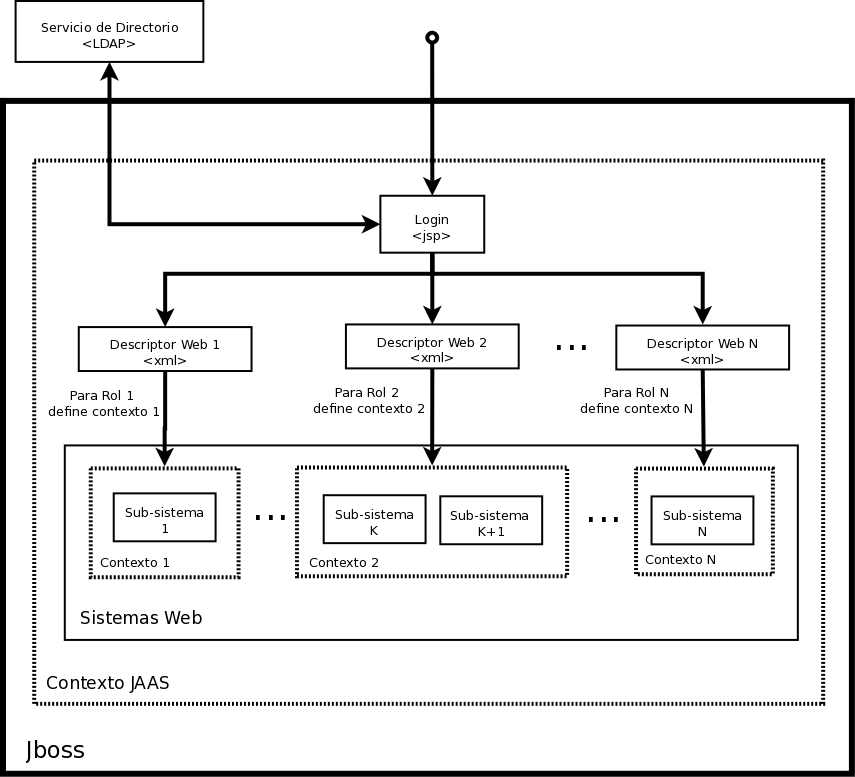
\includegraphics[scale=0.35]{img/diseno}

\subsection{Implementación}
\lstset{basicstyle=\tiny, breaklines=true, numbers=left,
frame=shadowbox, rulesepcolor=\color{black}}

	\subsubsection{Instalación de base de datos LDAP}
	\begin{enumerate}
		\item Bajar e instalar OpenLDAP.
		\item Configurar slapd.conf (hay que especificar el suffix, rootdn (usuario al
cual JBoss se conectará), rootpw, y opcionalmente el directorio.
		\item  Necesitamos tener los necesarios usuarios y grupos en LDAP que serán
utilizados en JBoss. Esto debe configurarse en el servidor LDAP previamente.
	\end{enumerate}

	\subsubsection{Implementación del SSO en JBoss}
	\begin{enumerate}
		\item Para activar SSO, simplemente activamos la opción en el archivo
de configuración de TomCat: JBOSS\_HOME/server/tu\_configuracion/deploy/jboss-web.deployer/server.xml.

	\end{enumerate}
	\subsubsection{Integración de LDAP utilizando JAAS en servidores web JBoss}
	\begin{enumerate}
			\item JBoss usa el LoginLdapModule para conectarse con LDAP.
			Configuramos la application-policy en el login-config.xml que puede ser encontrado en JBOSS\_HOME/server/default.conf. Esto permitirá a JBoss conectarse con el servidor LDAP y le dirá la estructura que debe tener, como su usuario, password y los roles que encontrará.
			\item Después de esto solo nos queda conectarnos a través de una
aplicación JAAS. En nuestro caso utilizamos un Servlet que probara la
conexión realizando ciertas consultas a la base de datos.
	\end{enumerate}
%	\item Integración con otros proyectos
%	\begin{enumerate}
%		\item 
%
%	\end{enumerate}
